% -*- coding:utf-8 -*-
\documentclass{standalone}
\usepackage{fontspec}
\setmainfont{Times New Roman}
\usepackage[UTF8]{ctex}
\usepackage{tikz}
\usepackage{amsmath}
\usetikzlibrary{matrix,calc,shapes,backgrounds,patterns,positioning,decorations.pathreplacing}
\begin{document}
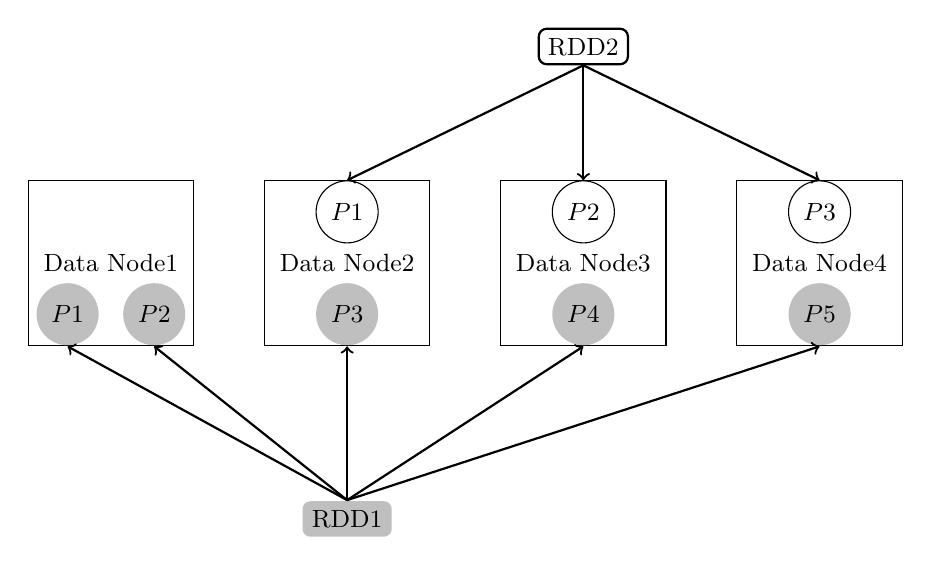
\begin{tikzpicture}
[partnode1/.style={circle, radius=0.1, thick, fill=lightgray},
partnode2/.style = {circle, radius=0.1,draw},
rddnode/.style={rectangle, rounded corners=1mm,thick, minimum width=1.8, minimum height=1},
]
\draw (0+0.2,0.2) rectangle (2.3,2.5-0.2);
\draw (3.5+0.2-0.5,0+0.2) rectangle (6-0.2-0.5,2.5-0.2);
\draw (7+0.2-0.5-0.5,0+0.2) rectangle (9.5-0.2-0.5-.5,2.5-0.2);
\draw (10.5+0.2-0.5-1,0+0.2) rectangle (13-0.2-0.5-1,2.5-0.2);
%node1
\node[partnode1](p11) at (0.7, 0.6){\small $P1$};
\node[partnode1](p12) at (1.8, 0.6){\small $P2$};
\node[] at (1.25, 1.25) {\small Data Node1};
%node2
\node[partnode1](p13) at (4.75-0.5, 0.6) {\small $P3$};
\node[partnode2](p21) at (4.75-0.5, 1.9) {\small $P1$};
\node at (4.75-0.5, 1.25) {\small Data Node2};
% node3
\node[partnode1](p14) at (8.25-0.5-0.5, 0.6) {\small $P4$};
\node[partnode2](p22) at (8.25-0.5-0.5, 1.9) {\small $P2$};
\node at (8.25-0.5-0.5, 1.25) {\small Data Node3};
% node 4
\node[partnode1](p15) at (11.75-0.5-1, 0.6) {\small $P5$};
\node[partnode2](p23) at (11.75-0.5-1, 1.9) {\small $P3$};
\node at (11.75-0.5-1, 1.25) {\small Data Node4};
% rdd
\node[rddnode,fill=lightgray](rdd1) at (4.25, -2) {\small RDD1};
\node[rddnode, draw](rdd2) at (7.25, 4){\small RDD2};
%draw line 
\draw[thick, ->] (rdd1.north) -- (p11.south);
\draw[thick, ->] (rdd1.north) -- (p12.south);
\draw[thick, ->] (rdd1.north) -- (p13.south);
\draw[thick, ->] (rdd1.north) -- (p14.south);
\draw[thick, ->] (rdd1.north) -- (p15.south);
\draw[thick, ->] (rdd2.south) -- (p21.north);
\draw[thick, ->] (rdd2.south) -- (p22.north);
\draw[thick, ->] (rdd2.south) -- (p23.north);
\end{tikzpicture}
\end{document}